\addcontentsline{toc}{section}{Приложение Б (обязательное)
  Модифицированная модель и \\ результаты её имитации}
\section*{ПРИЛОЖЕНИЕ Б \\ (обязательное) \\
  Модифицированная модель и результаты её имитации}

\pagestyle{fancy}
\fancyhf{}  % clear all header and footer fields
\fancyfoot[R]{\thepage}
\renewcommand{\headrulewidth}{0pt}
\renewcommand{\footrulewidth}{0pt}

\setlength{\headheight}{10mm}
\setlength{\headsep}{\baselineskip}
\chead{Продолжение приложения \Asbuk{section}}

\thispagestyle{plain}

\setcounter{section}{2}
\setcounter{figure}{0}
\setcounter{table}{0}
\setcounter{lstlisting}{0}

\lstinputlisting[caption=Исходный текст модифицированной GPSS-модели,
                 basicstyle=\scriptsize\ttfamily,
                 numberstyle=\scriptsize\ttfamily,
                 xleftmargin=10mm,
                ]{code/modif_calc.txt}

\begin{figure}[h!]
  \centering
  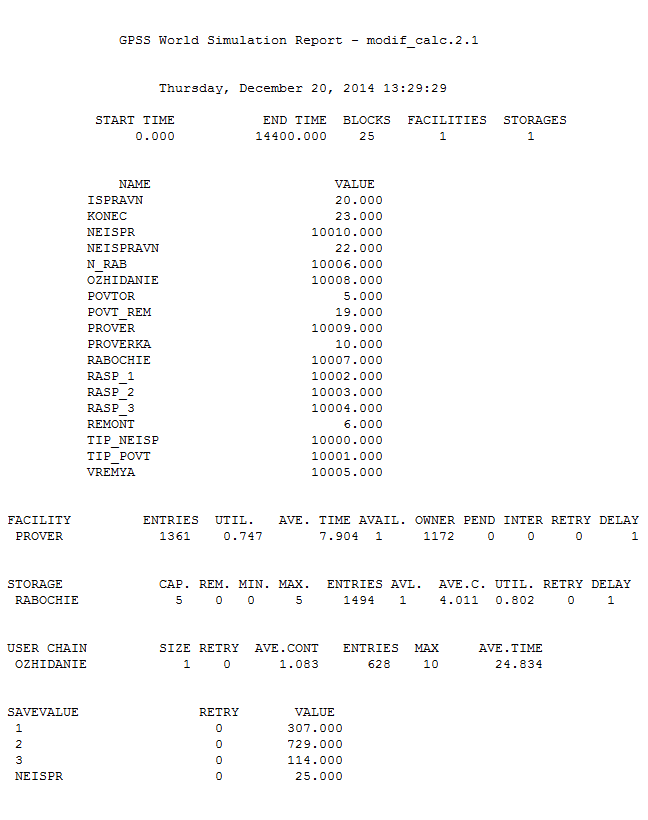
\includegraphics[width=150mm]{pic/modif_report}
  \caption{Файл статистики модифицированной GPSS-модели}
  \label{pic:modified_report}
\end{figure}
